\documentclass[conference]{IEEEtran}
\IEEEoverridecommandlockouts
% The preceding line is only needed to identify funding in the first footnote. If that is unneeded, please comment it out.
\usepackage{cite}
\usepackage{amsmath,amssymb,amsfonts}
\usepackage{algorithmic}
\usepackage{graphicx}
\usepackage{textcomp}
\usepackage{natbib}
\usepackage{float}
\usepackage{xcolor}
\def\BibTeX{{\rm B\kern-.05em{\sc i\kern-.025em b}\kern-.08em
    T\kern-.1667em\lower.7ex\hbox{E}\kern-.125emX}}
\begin{document}

\title{Machine Learning Approaches for Accurate Diamond Price Prediction\\
% {\footnotesize ECS-171 Final Project: \textbf{Group 21}}
\thanks{Final Project Report for ECS 171 - Group 21}
}

\author{
\IEEEauthorblockN{Aditya Mittal}
\IEEEauthorblockA{\textit{Department of Statistics} \\
\textit{University of California, Davis}\\
Davis, United States \\
adimittal@ucdavis.edu}
\and
\IEEEauthorblockN{Andrew Yeow}
\IEEEauthorblockA{\textit{Department of Computer Science} \\
\textit{University of California, Davis}\\
Davis, United States \\
XXX}
\and
\IEEEauthorblockN{Yifan Cui}
\IEEEauthorblockA{\textit{Department of Computer Science} \\
\textit{University of California, Davis}\\
Davis, United States \\
XXX}
\and
\IEEEauthorblockN{Nandini Koladi}
\IEEEauthorblockA{\textit{Department of Computer Science} \\
\textit{University of California, Davis}\\
Davis, United States \\
XXX}
\and
\IEEEauthorblockN{Eshan Toshniwal}
\IEEEauthorblockA{\textit{Department of Computer Science} \\
\textit{University of California, Davis}\\
Davis, United States \\
XXX}
}

\maketitle

\begin{abstract}
In 2023, the U.S. jewelry market was valued at 73.32 billion USD, with diamonds comprising a significant share. Predicting diamond prices accurately is essential for jewelers to make informed pricing decisions. This paper explores various machine learning algorithms, including linear regression, Random Forests, XGBoost, and neural networks, to predict diamond prices based on characteristics such as carat, cut, color, and clarity. Through exploratory data analysis, we identify key features influencing diamond prices and apply these insights to improve model performance. Our methodology includes rigorous model evaluation using metrics like Mean Squared Error (MSE), Mean Absolute Error (MAE), and R-squared (R²). By developing a robust predictive model, we aim to enhance pricing precision, benefiting both businesses and consumers in the diamond market.
\end{abstract}

\begin{IEEEkeywords}
Diamond pricing, machine learning, predictive modeling, neural network, decision trees
\end{IEEEkeywords}

\section{Introduction}

In 2023, the jewelry market in the United States was estimated to be worth 73.32 billion USD, with projections for 2024 reaching 96.61 billion USD \cite{a3}. Clearly, the market for jewelry is quite significant and continues to display steady growth. In particular, \emph{diamonds} account for a significant portion of this market, covering an estimated 50-60\% market share as compared to other precious stones such as gold, silver, etc \cite{a4}. Consequently, it becomes important for jewelers to adopt accurate methods to predict prices of these diamonds to better serve their consumers. In fact, businesses have began educating their sellers on essential qualities such as cut, color, carat weight, and clarity to make informed pricing decisions. As such, ensuring accurate price predictions becomes very important as it has significant financial implications on both businesses and consumers alike.

Given the importance of this task, it becomes crucial to develop methods that enable accurate prediction of prices for these diamonds. Machine learning, with its ability to learn patterns in data and make predictions, has become extremely popular in recent years across a wide range of applications \cite{a1}. Recent advancements in machine learning have introduced a range of algorithms, including linear regression, K-Nearest Neighbors, Random Forests, and the increasingly popular neural networks \cite{c1}. In this paper, we explore several different machine learning algorithms to accurately predict diamond prices based on several characteristics, including those mentioned above. The application of these predictions is widespread, as it can aid jewelers and marketers who aim to provide accurate pricing for consumers in the jewelry market.

Our dataset contains several essential features for diamond price prediction, such as the aforementioned carat, cut, color, clarity, etc \cite{a2}. Through exploratory data analysis (EDA), we aim to understand how these features relate to diamond prices. This analysis will help us answer questions about which features most significantly impact diamond prices and how we can leverage this information to create predictive models. Thus, our goal is to develop an accurate model for predicting diamond prices, enabling jewelers to make precise pricing decisions and enhancing the consumer purchasing experience. This paper details our methodology, including EDA and the application of various machine learning algorithms, to achieve this objective.

The outline of this paper is as follows: Section 2 discusses the historical perspective of machine learning and relevant algorithms as part of the literature review. Section 3 presents data description and exploratory data analysis. Sections 4 and 5 discuss the proposed methodology and results. Finally, the paper concludes with a discussion and future perspective in Section 6.

\section{Literature Review}

Machine learning is a rapidly developing field with a diverse range of algorithms tailored for various tasks. This section details important concepts surrounding the ML algorithms we will use. In particular, we discuss the historical context \& purpose of regression models, decision trees, and neural networks.

\subsection{Linear Regression} 

The most basic prediction model we explore is linear regression. This model fits a straight line between the response variable and its predictors, making it extremely simple and interpretable in terms of estimating the regression coefficients \cite{b10}. One major benefit of linear regression, compared to more complex models, is its efficiency and ease of interpretation, especially when the relationship between the dependent variable $Y$ and the independent variable(s) $X$ is approximately linear. For a single predictor $X$, the general form of a linear regression model is:

\[
    Y = \beta_0 + \beta_1 X + \epsilon
\]

Here, $\beta_0$ represents the intercept term, $\beta_1$ is the coefficient for X, and $\epsilon_1 \sim \mathcal{N}(0,\sigma_1^2)$. Note that $\epsilon_1$ is independent of the other predictor terms. Linear regression relies on several key assumptions, including linearity, independence, homoscedasticity, and normality of residuals \cite{b8}. The performance of a linear regression model can be evaluated using metrics such as $R^2$ and Mean Squared Error (MSE). Linear regression can be extended to more complex models, such as multiple linear regression, polynomial regression, and regularization methods (e.g., Ridge and Lasso regression) to handle more complex relationships and preventing overfitting.

A crucial part of linear regression is the minimization of the Residual Sum of Squares (RSS). The RSS measures the discrepancy between the observed data and the values predicted by the model:

\[
    \text{RSS} = \sum_{i=1}^n (y_i - \hat{y}_i)^2
\]

Minimizing the RSS through Ordinary Least Squares (OLS) provides the best-fitting line by ensuring the smallest possible error in predicting the response variable from the predictors. For further details on the mathematical foundations of OLS and RSS minimization, refer to Seber and Lee's comprehensive discussion on linear regression \cite{b9}. Linear regression has been extensively studied and applied across various fields \cite{b1, b2}. Additionally, Kutner et al. provide detailed discussions on the statistical assumptions, limitations, and diagnostics of linear regression models \cite{b8}.

\subsection{Decision Trees} 

The second major algorithm we review is decision trees. Decision trees are powerful tools for classification and regression tasks, especially with tabular data. These algorithms split the data into subsets based on the value of input features, creating a tree-like model of decisions. Decision trees can be prone to overfitting; however, ensemble methods such as Random Forests (Breiman, 2001) and Gradient Boosting Machines like XGBoost (Chen \& Guestrin, 2016) mitigate this issue by combining multiple trees to improve performance and robustness. Random forests, introduced by Breiman (2001), create a "forest" of multiple decision trees and aggregate their predictions. This method reduces variance and improves generalization by averaging multiple models . XGBoost, a popular implementation of gradient boosting, has been shown to deliver state-of-the-art performance in many machine learning competitions due to its efficiency and scalability.

Despite being recently popularized by the rise of AI applications, neural networks are actually a historical concept developed in the early 1980s. It resurgence was sparked by the rise of deep learning, with advancements in computational power to handle larger datasets.

\subsection{Neural Networks}

The foundation of modern neural networks was laid by the introduction of backpropagation by Rumelhart, Hinton, and Williams (1986) . Recently, deep learning has revolutionized fields such as image recognition, natural language processing, and game playing. LeCun, Bengio, and Hinton (2015) provide a seminal review on the principles and advancements in deep learning. A neural network contains many hyperparameters, and there are several elements to finding the best set of such values. Grid search is a systematic approach for hyperparameter tuning, where a predefined set of hyperparameters is evaluated exhaustively to identify the optimal configuration for a machine learning model. Bergstra and Bengio (2012) introduced grid search as a fundamental method for hyperparameter optimization. They highlighted its importance in efficiently exploring the hyperparameter space and provided insights into its limitations, such as scalability and computational cost. For a comprehensive discussion on hyperparameter optimization techniques, see the review by Loshchilov and Hutter (2019).

The Adam optimizer, short for Adaptive Moment Estimation, is a widely used optimization algorithm for training deep neural networks. It combines the advantages of both adaptive learning rate methods and momentum-based optimization techniques, offering fast convergence and robustness to noisy gradients. Kingma and Ba (2014) introduced the Adam optimizer, presenting it as an extension of the stochastic gradient descent with adaptive learning rates. They demonstrated its effectiveness in training deep learning models across various tasks, including image classification, natural language processing, and reinforcement learning. Adam maintains adaptive learning rates for each parameter by computing individual learning rates based on the first and second moments of the gradients. This adaptive behavior allows Adam to automatically adjust the learning rate during training, leading to improved convergence and generalization performance.

In conclusion, grid search and the Adam optimizer are essential components of the machine learning and deep learning toolkit. While grid search provides a systematic approach for hyperparameter tuning, Adam offers an efficient optimization algorithm for training deep neural networks. Understanding their strengths, limitations, and best practices is crucial for effectively applying these techniques in practical scenarios.


\section{Dataset Description and Exploratory Data Analysis}

The \emph{diamond prices} dataset contains detailed information about 54,000 diamonds, including their prices and various characteristics \cite{a2}. The predictor variables in this dataset are as follows: i) \textbf{Carat}: Represents the weight of the diamond, ranging from 0.2 to 5.01 carats. ii) \textbf{Cut Quality}: Categorized as Fair, Good, Very Good, Premium, or Ideal, indicating the craftsmanship involved in shaping the diamond. iii) \textbf{Color}: Graded from J (worst) to D (best), reflecting the hue and saturation of the stone. iv) \textbf{Clarity}: Measures how clear the diamond is, with grades ranging from I1 (worst), SI2, SI1, VS2, VS1, VVS2, VVS1, to IF (best). v) \textbf{Dimensions}: Captured by the length (x), width (y), and depth (z) in millimeters, with ranges of 0–10.74 mm, 0–58.9 mm, and 0–31.8 mm, respectively. vi) \textbf{Depth Percentage}: Ranges from 43\% to 79\%. vii) \textbf{Table}: Represents the width of the top of the diamond relative to its widest point, ranging from 43\% to 95\%. The dataset does not contain any missing values, so we do not need to address missing data in the exploratory data analysis step.

\subsection{Exploratory Data Analysis}

To explore the dataset further and understand the relationships between these features and diamond prices, we will conduct exploratory data analysis (EDA). First, we visualize the distribution of each continuous feature, such as carat, length (x), width (y), depth (z), depth percentage, and table, to understand their spread and central tendencies. A table will highlight the mean, median, and standard deviation statistics of each feature, providing insights into their individual magnitudes and spread. Second, pairwise scatter plots display the relationship between each continuous feature and diamond price, helping to identify potential trends and correlations. Third, the correlation heat-map presents Pearson correlation relationships between continuous features, helping identify features most correlated with price. Finally, we create histograms of categorical features like cut, color, and clarity to understand their distributions. These visualizations provide insights into the structure of the data, highlight any anomalies, and help with subsequent modeling efforts to predict diamond prices effectively.

\begin{figure}[H]
    \centering
    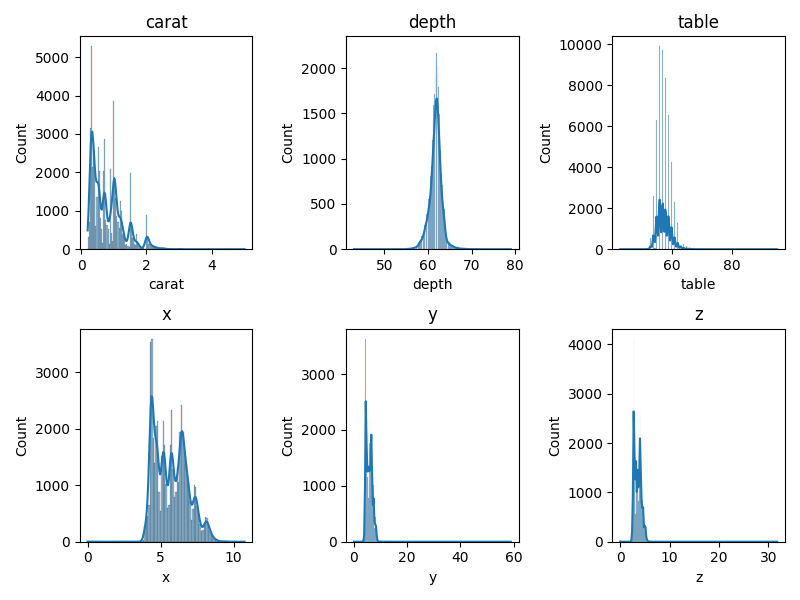
\includegraphics[width=0.8\linewidth]{Figure_1.png}
    \caption{Distribution Plot of Continuous Features. Reveals trends in data such as skewness, location of outliers, etc.}
    \label{fig:image_label}
\end{figure}

The distribution of continuous predictors highlight potential skewness in our dataset. For instance, the predictor \emph{carat} suggests potential skewness to the right – with many upper outliers – as evidenced by its distribution plot. This trend holds true for features \emph{y} and \emph{z} as well. These plots suggest that our dataset may contain a significant number of upper outliers, which we will consider removing in the data pre-processing stage. To further gain insight on the distribution of our features, the table below summarizes the mean, median, and standard deviation of the continuous features:

\begin{table}[H]
    \centering
    \caption{Mean, Median, Standard Dev. of Continuous Features}
    \label{tab:example_table}
    \begin{tabular}{|c|c|c|c|}
        \hline
        Feature & Mean & Median & Standard Dev. \\
        \hline
        Carat & 0.797 & 0.70 & 0.474 \\
        \hline
        Depth & 61.749 & 61.80  & 1.432 \\
        \hline
        Table & 57.457 & 57.00 & 2.234 \\
        \hline
        X & 5.731 & 5.70 & 1.122 \\
        \hline
        Y & 5.734 & 5.71 & 1.142 \\
        \hline
        Z & 3.538 & 3.53 & 0.705 \\
        \hline
    \end{tabular}
\end{table}

From our table, we can observe that the mean and median values for most features are relatively close, indicating that the data distributions may not actually be as heavily skewed for most variables. However, the standard deviation values highlight the variability within each feature, such as carat and dimensions (x, y, z), display considerable spread. This variability and potential skewness, especially in the carat feature from the plots, could influence our predictive algorithms. Next, we will create pairwise scatter-plots to identify trends between diamond prices and the features.

\begin{figure}[H]
    \centering
    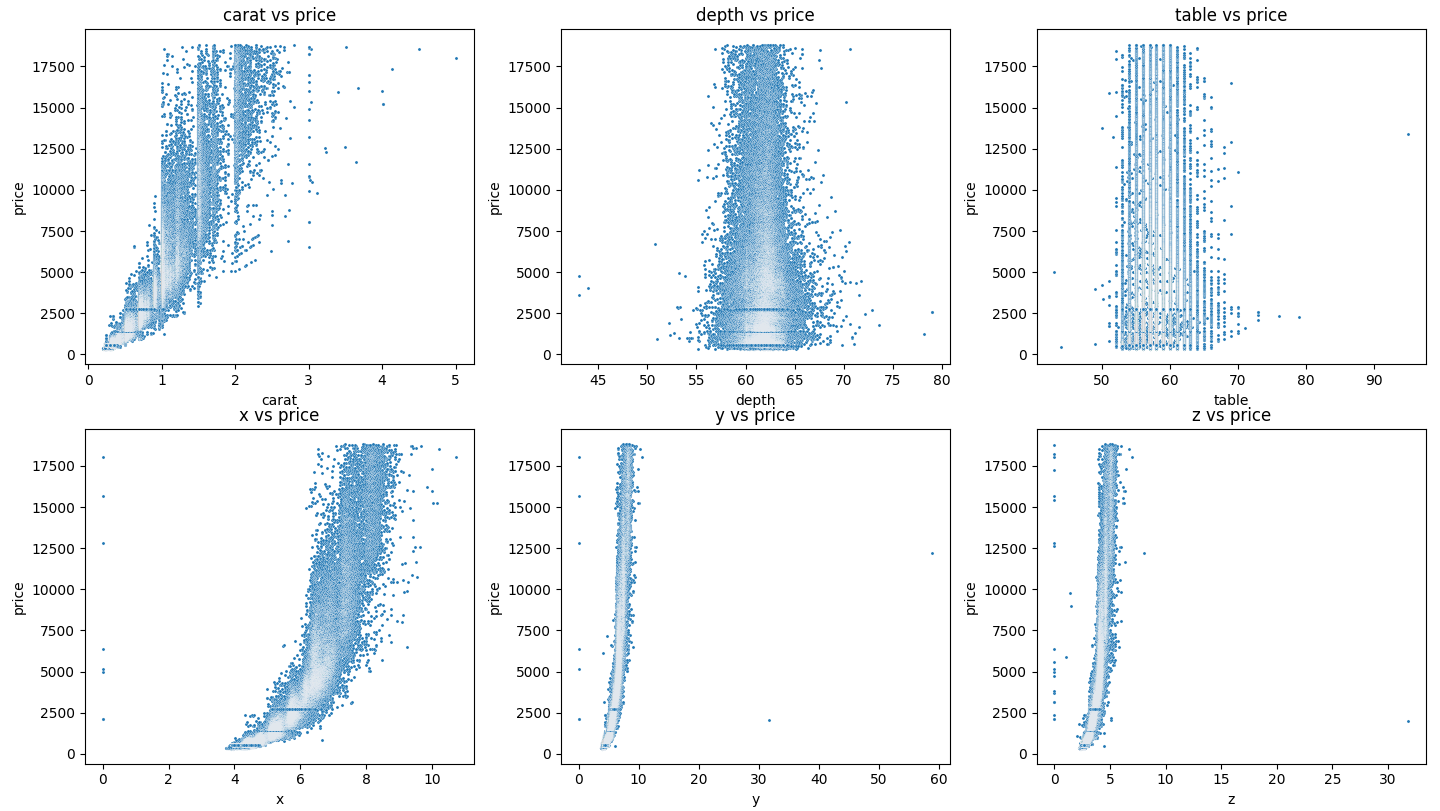
\includegraphics[width=0.8\linewidth]{Figure_4.png} % Replace "example-image" with the filename of your image
    \caption{Pair-wise Scatterplots for Each Feature vs. Diamond Price}
    \label{fig:image_label}
\end{figure}

From the scatterplots of each feature against the response variable, we observe a quadratic relationship between the features, carat, x, y, and z, with respect to the the response variable price. This suggests that a polynomial regression model might be suitable for our dataset in addition to a linear regression model. Thus, we will evaluate the polynomial regression model's performance on the dataset compared to traditional linear regression. Next, we will also analyze the correlations between these continuous features and the target variable, price, to determine the most influential predictors. This will allow us to identify the most relevant features and also potential multicollinearity and interactions.

\begin{figure}[H]
    \centering
    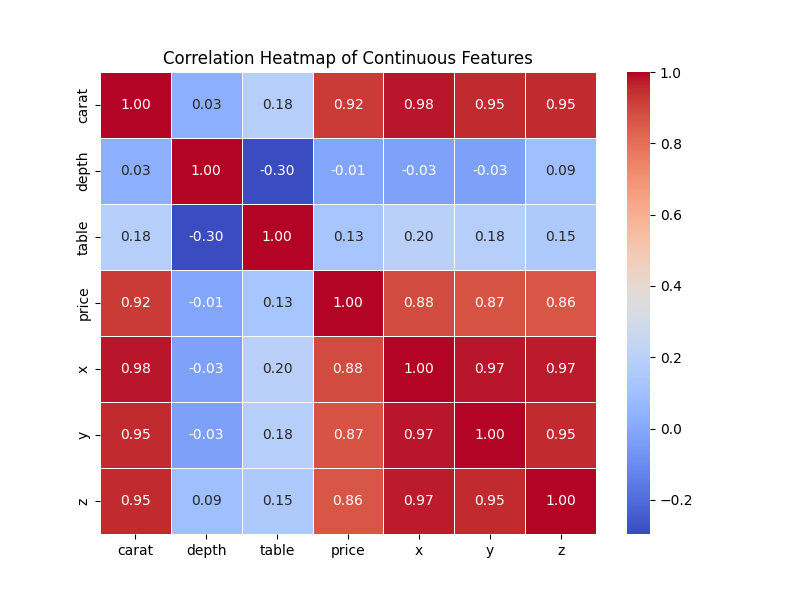
\includegraphics[width=0.8\linewidth]{Figure_3.png} % Replace "example-image" with the filename of your image
    \caption{Correlation Heat-Map for Continous Features vs Diamond Price}
    \label{fig:image_label}
\end{figure}

Based on the results of our correlation heatmap, the feature \emph{Carat} appears to be highly correlated with price, with a correlation coefficient of 0.92. Similarly, it is correlated with dimension features \emph{x}, \emph{y}, and \emph{z}. This makes sense, as carat weight would directly relate to diamond size. Thus, this plot suggests that Carat (and potentially dimensions) are the strongest predictors for diamond price. We showcase data preprocessing methods for outlier removal using carat below. On the other hand, both depth percentage and table have almost zero correlation, indicating that they do not have much association with diamond prices. Thus, this heatmap is insightful in identifying the key predictors for diamond prices and guiding our feature selection process. Next, we will examine histograms for the distribution of categorical features cut, clarity, and color:

\begin{figure}[H]
    \centering
    \includegraphics[width=0.8\linewidth]{figure_5.png} % Replace "example-image" with the filename of your image
    \caption{Historgram for the distribution of categorical features: Cut, Clarity, and Color }
    \label{fig:image_label}
\end{figure}

The histogram of the categorical variables displays their frequencies. Upon initial analysis of the plot, we observe that the cut category "Ideal" appears most frequently, followed by "Premium" and "Very Good," while the "Fair" cut appears least frequently. The distribution of color appears to be well spread, with all colors represented. Regarding clarity, categories such as "I1" and "IF" have relatively few observations compared to others. With this, our exploratory data analysis step has provided valuable insights into the structure of the dataset and identify patterns among the features. We will now proceed with data pre-processing before implementing our machine learning algorithms.

\subsection{Data Pre-Processing} 

Before implementing the machine learning algorithms, we conducted several pre-processing steps on our dataset. First, considering the ordinality present in each of our categorical features, we implemented label encoding to convert these features into numeric representations. The mappings for each categorical feature were defined as follows:

\begin{table}[htbp]
    \centering
    \caption{Label Encodings for Categorical Features}
    \resizebox{\columnwidth}{!}{
        \begin{tabular}{|l|l|}
            \hline
            \textbf{Feature} & \textbf{Encoding} \\
            \hline
            Cut & 'Fair': 0, 'Good': 1, 'Very Good': 2, 'Premium': 3, 'Ideal': 4 \\
            Color & 'J': 0, 'I': 1, 'H': 2, 'G': 3, 'F': 4, 'E': 5, 'D': 6 \\
            Clarity & 'I1': 0, 'SI2': 1, 'SI1': 2, 'VS2': 3, 'VS1': 4, 'VVS2': 5, 'VVS1': 6, 'IF': 7 \\
            \hline
        \end{tabular}
    }
    \label{tab:label_encodings}
\end{table}

Next, to standardize our data and balance the scale of our features, we applied z-score transformation. This transformation ensures that all our features have a mean of 0 and a standard deviation of 1, thereby balancing the scales among features. This is particularly beneficial for algorithms such as neural networks. Finally, we proceeded to remove outliers. Since carat was our most highly correlated predictor, we used it as the feature to identify and remove outliers using the 1.5 times the interquartile range (IQR) calculation. Approximately 3.9\% of the dataset was removed through this process, leaving us with 51,800 rows of data. The boxplots for each feature post outlier removal are shown below:

\begin{figure}[H]
    \centering
    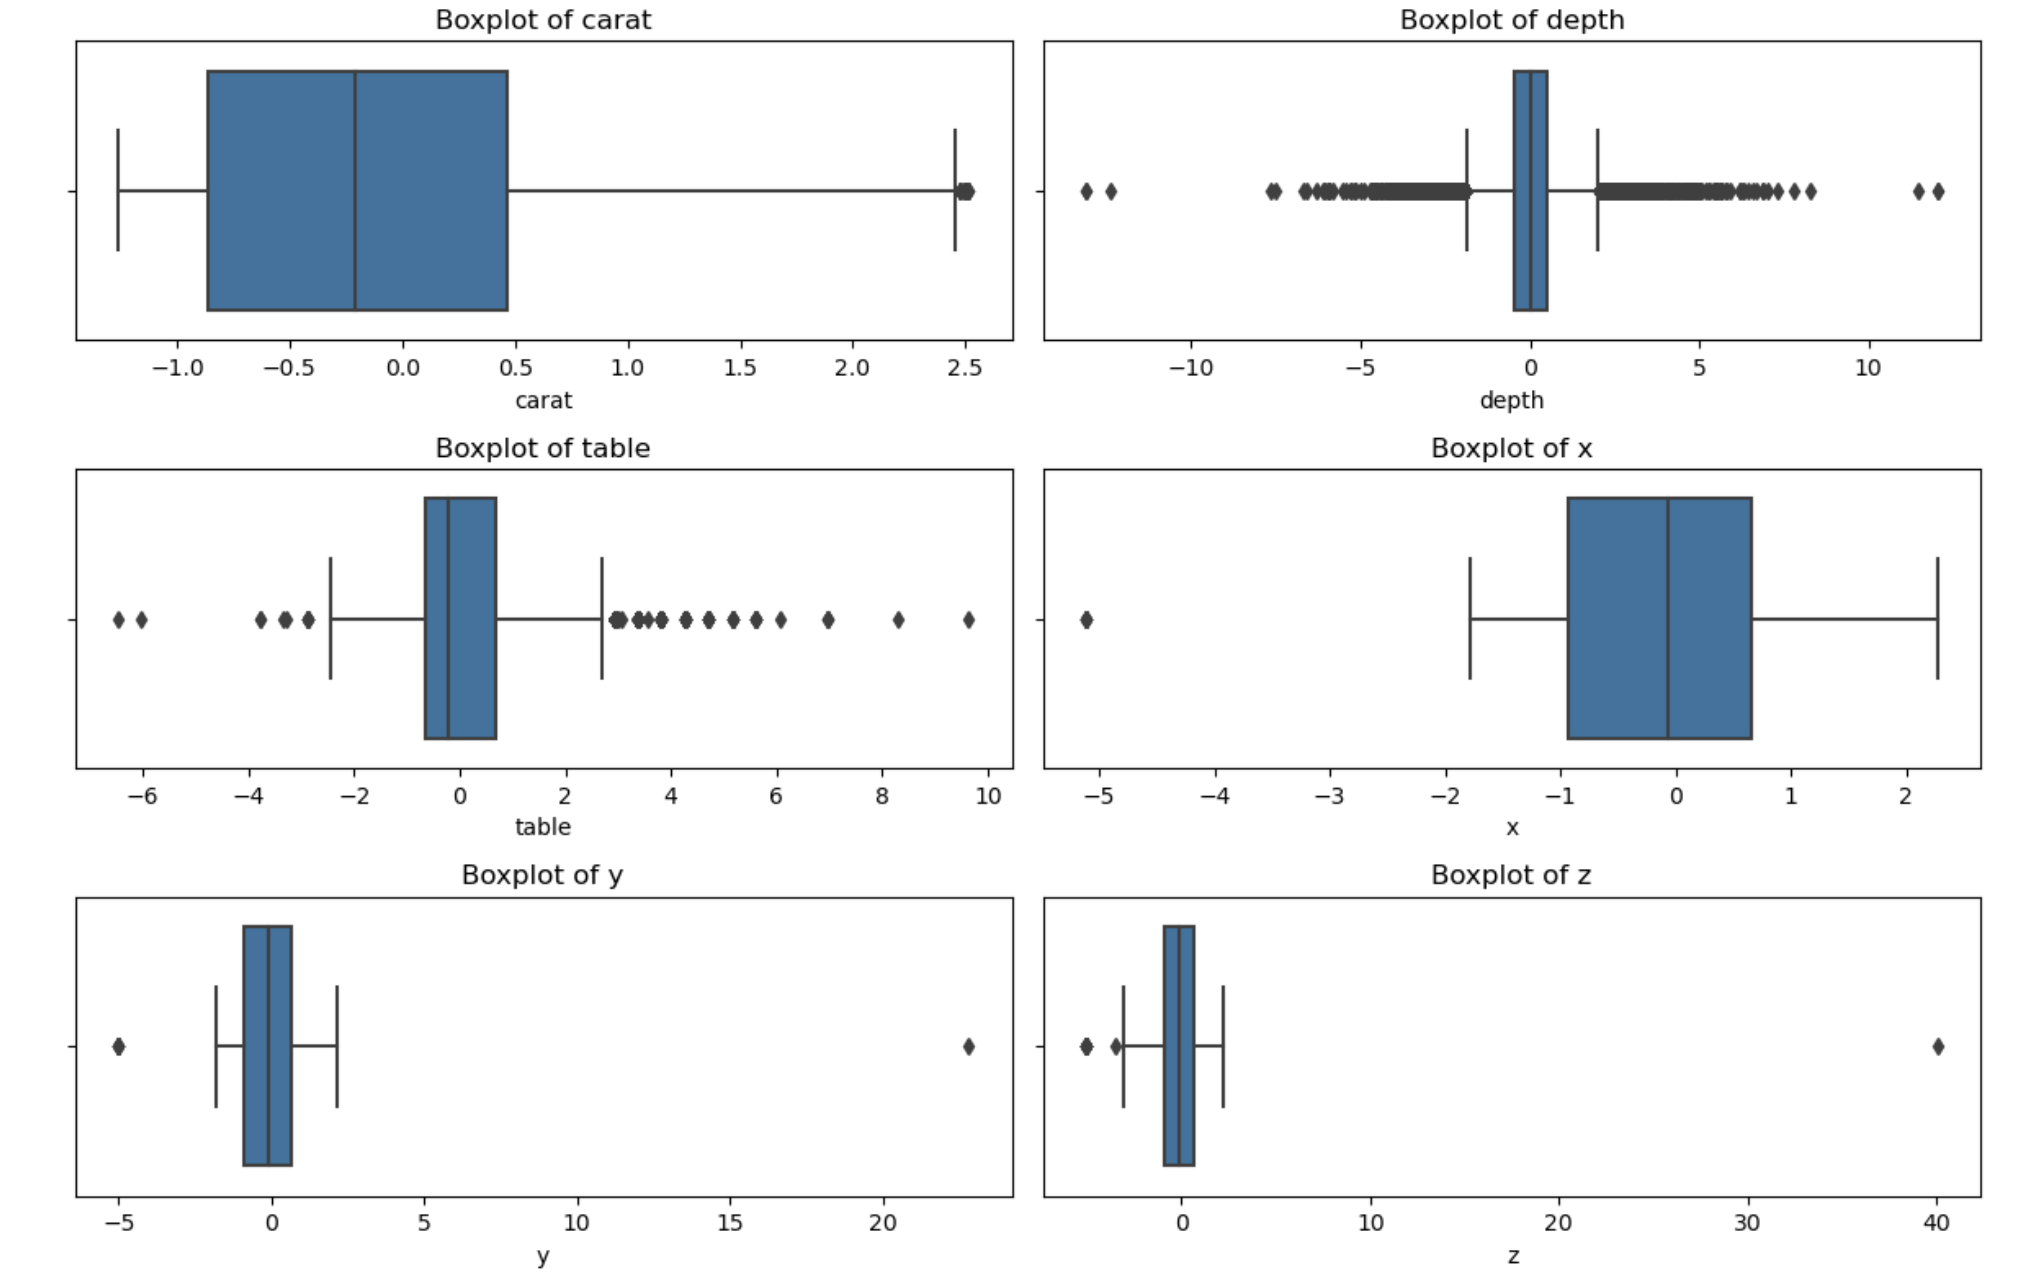
\includegraphics[width=0.8\linewidth]{boxplot.png} % Replace "example-image" with the filename of your image
    \caption{Boxplots of Features Post-Outlier Removal}
    \label{fig:boxplots}
\end{figure}

The boxplots indicate that outliers were removed for carat, while several other features such as depth and table still exhibit upper values. Since these features are not highly correlated with our response variable, we decided to keep them as is and proceed with this cleaned version of the dataset.

\section{Proposed methodology}

In this paper, we explore the predictive capabilities of several machine learning algorithms, ranging from linear regression and polynomial regression to decision trees and artificial neural networks. Our approach involves multiple steps to build and evaluate models that can accurately predict diamond prices based on various features.

We begin with traditional linear regression to fit a straight-line model between diamond prices and the aforementioned features. This initial step helps us gain intuition about the relationship between the features and diamond prices using a simple model. Recognizing that the price exhibited a quadratic relationship with carat and diamond dimensions, we extend our analysis to polynomial regression by including squared terms of these features. This allows us to capture potential nonlinear relationships and assess whether polynomial regression outperforms traditional linear regression.

For decision tree-based models, we employ two powerful algorithms: Random Forests and XGBoost. Random Forests aggregate the predictions of multiple decision trees to enhance accuracy and reduce overfitting. XGBoost, a gradient boosting algorithm, further refines predictions by optimizing the model iteratively to minimize errors. These models are well-suited for capturing complex interactions between features and are expected to perform robustly on our dataset.

Finally, we explore the use of artificial neural networks (ANNs) for generating predictions. To optimize our ANN, we conduct a grid search for hyperparameter tuning, ensuring we select the best set of parameters for our model. Our neural network architecture consists of a 3-layer ANN with 64 neurons in the first hidden layer, using the ReLU activation function. The output layer also employs the ReLU activation function, as our task involves regression.

To evaluate the performance of our models, we will compare their results using several metrics, including Mean Squared Error (MSE), Mean Absolute Error (MAE), and R-squared (R²). These metrics will help us determine the accuracy and reliability of each model on testing data. By comparing these measures, we aim to identify the most effective algorithm for predicting diamond prices, providing valuable insights for jewelers and marketers in the industry.

Through this comprehensive methodology, we seek to develop an accurate and robust model for predicting diamond prices, leveraging the strengths of various machine learning techniques to achieve the best possible performance.

\section{Experimental results and evaluation}

\section{Conclusion}

In this study, we investigated various machine learning algorithms to predict diamond prices based on key characteristics such as carat, cut, color, clarity, and dimensions. Our analysis demonstrated that advanced machine learning techniques, particularly Random Forests, XGBoost, and neural networks, significantly outperformed traditional linear regression models in terms of predictive accuracy. The exploratory data analysis revealed that carat is the most influential feature, with strong correlations to price and other dimensions. 

Our findings suggest that leveraging these advanced models can provide jewelers and consumers with more accurate pricing, enhancing decision-making and market transparency. Future work can explore integrating additional features, refining model hyperparameters, and applying these models to other datasets to generalize our findings further.

By adopting robust machine learning methodologies, the diamond industry can benefit from more precise pricing strategies, ultimately leading to improved market efficiency and customer satisfaction.

\begin{thebibliography}{00}
\bibitem{a1} Kino, S., Hsu, Y.-T., Shiba, K., Chien, Y.-S., Mita, C., Kawachi, I., and Daoud, A. (2021). A scoping review on the use of machine learning in research on social determinants of health: Trends and research prospects. SSM - Population Health, 15, 100836.
\bibitem{c1} Sarker, I.H. Machine Learning: Algorithms, Real-World Applications and Research Directions. SN COMPUT. SCI. 2, 160 (2021). https://doi.org/10.1007/s42979-021-00592-x
\bibitem{a2} Agrawal, S. (2017a, May 25). Diamonds. Kaggle. https://www.kaggle.com/datasets/shivam2503/diamonds 
\bibitem{a3} U.S. jewelry market size and share: Industry Report, 2030. U.S. Jewelry Market Size And Share | Industry Report, 2030. (n.d.). https://www.grandviewresearch.com/industry-analysis/us-jewelry-market-report 
\bibitem{a4} Diamond Jewelry Market Size \& Share Analysis Report, 2030. (n.d.). https://www.grandviewresearch.com/industry-analysis/diamond-jewelry-market-report 
\bibitem{b1} Weisberg, S. (2005). Applied Linear Regression. Wiley.
\bibitem{b2} Chatterjee, S., \& Hadi, A. S. (2015). Regression Analysis by Example. Wiley.
\bibitem{b3} Breiman, L. (2001). Random Forests. Machine Learning, 45(1), 5-32.
\bibitem{b4} Chen, T., \& Guestrin, C. (2016). XGBoost: A Scalable Tree Boosting System. In Proceedings of the 22nd ACM SIGKDD International Conference on Knowledge Discovery and Data Mining (pp. 785-794).
\bibitem{b5} Rumelhart, D. E., Hinton, G. E., \& Williams, R. J. (1986). Learning representations by back-propagating errors. Nature, 323(6088), 533-536.
\bibitem{b6} LeCun, Y., Bengio, Y., \& Hinton, G. (2015). Deep learning. Nature, 521(7553), 436-444.
\bibitem{b7}Vaswani, A., Shazeer, N., Parmar, N., Uszkoreit, J., Jones, L., Gomez, A. N., Kaiser, Ł., \& Polosukhin, I. (2017). Attention is all you need. In Advances in Neural Information Processing Systems (pp. 5998-6008).
\bibitem{b8}Michael Kutner, Christopher Nachtsheim, John Neter, and William Li. Applied Linear Statistical Models. 1974.
\bibitem{b9}Seber, G. A. F., \& Lee, A. J. (2012). Linear Regression Analysis. Hoboken, NJ: John Wiley \& Sons. 
\bibitem{b10} Wright, John T. "Linear Regression Analysis." British Medical Journal, vol. 310, no. 6977, 1995, pp. 1120-1124. BMJ Group
\end{thebibliography}
\vspace{12pt}






\end{document}
